\chapter{System design and construction}
\label{chap:construccio}

\section{Introduction}
\label{sec:introduccio}

This document describes the design, construction and in-flight validation of a complete precision aerial photogrammetry system (drone \emph{surveying}): an RTK GNSS base of its own, a UAV with two GNSS receivers and a camera with hot-shoe timing, and a ground station that links them.

The goal is centimetre-level geotagging of aerial photographs ($\leq 2$~cm horizontal, $\leq 3$~cm vertical) to produce survey-grade orthomosaics and digital surface models, with a total hardware cost of around €2,150 --~a fraction of the cost of a DJI P4 RTK or of an Emlid~+~UAV set~-- and with full control over the \emph{firmware}, the corrections and the data flow.

The system is divided into three subsystems:
\begin{itemize}
    \item \textbf{RTK GNSS base}: fixed station that generates RTCM3 corrections.
    \item \textbf{UAV (\emph{rover})}: drone with two GNSS receivers for RTK positioning and \emph{moving baseline} heading.
    \item \textbf{Ground station (GS)}: telemetry link and relay of the corrections to the drone.
\end{itemize}

The document is organised in four blocks: design and construction (this chapter), the operation manual and procedures (\cref{chap:manual}), the flight-test and tuning campaign (\cref{chap:proves-vol}) and the photogrammetry flights that result from it (\cref{chap:vols-prova}).

\section{Architecture and data flow}
\label{sec:arquitectura}

The chosen architecture uses the base to serve RTCM3 corrections over local WiFi (\emph{access point} mode) through a TCP server of its own, without NTRIP. A direct base~$\rightarrow$~drone radio link was discarded to simplify the system (a single radio channel to the drone) and to gain resilience in rural areas without mobile coverage.

\begin{figure}[H]
    \centering
    \resizebox{\linewidth}{!}{%
    \begin{tikzpicture}[
        box/.style={draw, rounded corners=2pt, align=center, font=\small, minimum height=10mm, minimum width=27mm, fill=blue!5},
        arr/.style={-{Stealth[length=2mm]}, thick},
        grp/.style={draw, dashed, rounded corners=4pt, inner sep=4mm, gray},
        node distance=8mm and 17mm]
        \node[box] (ant) {Multiband\\antenna};
        \node[box, right=of ant] (f9b) {ZED-F9P\\(base, \emph{survey-in})};
        \node[box, right=of f9b] (pi) {Raspberry Pi\\TCP server};
        \node[box, below=16mm of pi] (gs) {Mission Planner\\(ground station)};
        \node[box, left=of gs] (rfdg) {RFD868x\\(GS side)};
        \node[box, below=16mm of rfdg] (rfdu) {RFD868x\\(drone side)};
        \node[box, right=of rfdu] (fc) {Flight controller\\(Kakute H7, EKF3)};
        \node[box, right=of fc] (gnss) {2$\times$ ZED-F9P\\\emph{moving baseline}};
        \node[box, below=10mm of fc] (cam) {Sony $\alpha$6000\\MAP2 + SYNC2};
        \draw[arr] (ant) -- (f9b);
        \draw[arr] (f9b) -- node[above, font=\scriptsize] {RTCM3} (pi);
        \draw[arr] (pi) -- node[right, font=\scriptsize] {WiFi} (gs);
        \draw[arr] (gs) -- node[above, font=\scriptsize] {USB} (rfdg);
        \draw[arr] (rfdg) -- node[right, font=\scriptsize] {868~MHz} (rfdu);
        \draw[arr] (rfdu) -- node[above, font=\scriptsize] {MAVLink} (fc);
        \draw[arr, <->] (fc) -- node[above, font=\scriptsize] {UART} (gnss);
        \draw[arr, <->] (fc) -- node[right, font=\scriptsize] {PWM / hot shoe} (cam);
        \begin{scope}[on background layer]
            \node[grp, fit=(ant)(f9b)(pi), label={[font=\small, gray]above:RTK base}] {};
            \node[grp, fit=(rfdu)(fc)(gnss)(cam), label={[font=\small, gray]above:UAV}] {};
        \end{scope}
    \end{tikzpicture}}
    \caption{Block diagram of the system and flow of the RTCM3 corrections.}
    \label{fig:diagrama-blocs}
\end{figure}

\subsection{Complete data flow}

\begin{enumerate}[label=\arabic*.]
    \item The multiband antenna receives L1/L2/L5 (GPS, GLONASS, Galileo, BeiDou).
    \item The base \textbf{ZED-F9P} (\emph{survey-in} mode in every session, \cref{sec:protocol-camp}) generates \textbf{RTCM3} messages (1005, 1074, 1084, 1094, 1124 and 1230) at 1~Hz. Message 1005, with the base position, is only emitted when the \emph{survey-in} is valid.
    \item The \textbf{Raspberry Pi} receives these messages over USB (serial port of the simpleRTK2B Pro receiver) and redistributes them as they arrive through the TCP server on port 5000, over WiFi AP.
    \item The \textbf{GS} (Mission Planner / QGroundControl at the pilot's side) connects to the TCP server and forwards the RTCM3 stream to the drone over MAVLink (\texttt{GPS\_RTCM\_DATA}) through the \textbf{RFD868x} pair.
    \item On the drone, the primary F9P receives the corrections, computes the RTK position and, in \emph{moving baseline} mode, generates RTCM 4072.x for the secondary to derive the \emph{heading}.
    \item The \textbf{FC} integrates the RTK position and the GNSS \emph{yaw} in the EKF3 for navigation and geotagging.
\end{enumerate}

\section{Design decisions}
\label{sec:decisions}

\begin{description}
    \item[Moving baseline with 2$\times$ ZED-F9P] instead of a UM982 with native \emph{heading}. The F9P is better documented, has more community support and is interchangeable between base and UAV. It provides GPS-for-yaw, which makes it possible to do without the magnetic compass --~an important advantage on \emph{frames} with a lot of current.
    \item[RFD868x for the GS$\leftrightarrow$UAV link] at 868~MHz (European band) it allows up to 500~mW EIRP and a range above 40~km. Always the European 868 version (never 915 or 433).
    \item[Local TCP server over WiFi] robust in the absence of mobile coverage; in practice it is almost always operated locally (park the vehicle, set up the tripod next to it and fly).
    \item[Hot-shoe feedback (Seagull SYNC2)] solves the variable shutter latency ($\sim$100~ms equals 1.5~m of error at 15~m/s). Without this \emph{feedback} there is no real centimetre-level precision in the geotagging; \cref{sec:retard-obturador} quantifies the effect.
    \item[Optional PPK post-processing] logging of raw \texttt{UBX} data at the base and on the drone, which gives a solution independent of the quality of the real-time RTK link.
\end{description}

\section{Bill of materials}
\label{sec:materials}

The hardware of the system has a total cost of €2,150.

\subsection{Drone}

\begin{table}[H]
    \centering
    \caption{Drone components (UAV/\emph{rover})}
    \label{tab:materials-dron}
    \begin{tabular}{lll}
        \toprule
        Component & Model & Approx. cost \\
        \midrule
        \emph{Frame} & S500 (Quad X, 500~mm between axes) & €35 \\
        Motors (4$\times$) & Pilotix 2808, 1100~KV & €60 \\
        ESC & Hobbywing XRotor 65A 4-in-1 (DShot) & €30 \\
        FC & Holybro Kakute H7 (STM32H7) & €55 \\
        GPS (2$\times$) & Holybro H-RTK F9P Helical & €510 (€255 each) \\
        Telemetry & RFD868x EU 500~mW (drone + GS pair) & €363 \\
        RC & Radiomaster XR1 Nano ELRS dual-band & €16 \\
        Battery & Gaoneng GNB 6S 4000~mAh 70C & €70 \\
        \bottomrule
    \end{tabular}
\end{table}

\begin{description}
    \item[Pilotix 2808 motors, 1100~KV] moderate KV for 6S, intended for 8-inch propellers (\cref{tab:kv-compatibilitat}) with the additional payload of the RTK~+~camera system, instead of the high KV typical of \emph{freestyle}, which sacrifice efficiency for speed. The 7-inch propellers of the initial build were used for availability, not by design (\cref{subsec:propulsor-inicial}).
    \item[Hobbywing XRotor 65A 4-in-1 ESC (DShot)] current margin for the additional weight; bidirectional DShot gives per-motor RPM telemetry, useful for vibration diagnosis; the 4-in-1 format simplifies the power wiring.
    \item[Holybro Kakute H7 FC (STM32H7)] enough UART ports for the whole architecture without any expansion (2$\times$F9P, RFD868x, ELRS RC, ESC telemetry, USB) and native ArduPilot support for \emph{moving baseline} GPS and DShot.
    \item[Holybro H-RTK F9P Helical GPS (2$\times$)] integrated module (helical antenna + F9P \emph{breakout}) already designed for \emph{moving baseline} with ArduPilot; avoids having to design and match antenna and \emph{breakout} separately.
    \item[RFD868x telemetry] full justification in \cref{sec:decisions}.
    \item[Radiomaster XR1 Nano ELRS RC] minimum size and weight so as not to penalise the payload; low-latency ELRS complements the RFD868x, which carries the MAVLink/RTCM data but not the flight control.
    \item[Gaoneng 6S 4000~mAh 70C battery] 6S for better voltage efficiency with the additional consumption (GPS, telemetry, camera); 70C gives enough peak-current margin with the 4 motors at full load.
\end{description}

\subsection{GNSS base}

\begin{table}[H]
    \centering
    \caption{RTK base components}
    \label{tab:materials-base}
    \begin{tabular}{lll}
        \toprule
        Component & Model & Approx. cost \\
        \midrule
        GNSS & ArduSimple simpleRTK2B Pro (ZED-F9P) & €126 \\
        Antenna & BD900 GNSS (multiband) & €43 \\
        SBC & Raspberry Pi Zero W & €35 \\
        Power & Waveshare UPS HAT + 2$\times$ 18650 3500~mAh & €47 \\
        \bottomrule
    \end{tabular}
\end{table}

\begin{description}
    \item[simpleRTK2B Pro GNSS (ZED-F9P)] development board with USB and an SMA antenna connector, with the same chip as the drone receivers, which gives interchangeability and a shared configuration and \emph{firmware} (\cref{sec:decisions}).
    \item[BD900 GNSS antenna (multiband)] necessary to receive the two bands and the multiple constellations used by the ZED-F9P, a requirement for the \emph{survey-in} to converge (\cref{sec:protocol-camp}).
    \item[Raspberry Pi Zero W] small size and low consumption for field use on battery, with enough capacity to distribute the corrections through the TCP server and act as a WiFi access point (NetworkManager).
    \item[UPS HAT + 2$\times$18650 power] base endurance independent of the mains in the field, with protection against cuts during logging.
\end{description}

\subsection{Ground station}

\begin{table}[H]
    \centering
    \caption{Ground station (GS) components}
    \label{tab:materials-gs}
    \begin{tabular}{lll}
        \toprule
        Component & Model & Approx. cost \\
        \midrule
        Transmitter & Radiomaster TX16S (or similar) ELRS & €167 \\
        Telemetry & RFD868x (GS side, included in the pair) & -- \\
        Laptop / tablet & Own, with Mission Planner & -- \\
        \bottomrule
    \end{tabular}
\end{table}

The transmitter and the RFD868x pair are standard items with no specific design decision. The only additional element of the GS is the laptop or tablet with Mission Planner or QGroundControl, which bridges the base TCP server and the MAVLink stream to the drone (\cref{sec:arquitectura}).

\subsection{Camera (mapping module)}

\begin{table}[H]
    \centering
    \caption{Camera module for photogrammetry}
    \label{tab:materials-camera}
    \begin{tabular}{lll}
        \toprule
        Component & Model & Approx. cost \\
        \midrule
        Body & Sony $\alpha$6000 (24~MP APS-C, second hand) & €200 \\
        Lens & TTArtisan 25~mm f/2 APS-C, manual focus & €71 \\
        \emph{Trigger} & Seagull MAP2 (fires by PWM) & €30 \\
        \emph{Feedback} & Seagull SYNC2 (hot shoe, X-sync $\rightarrow$ FC) & €30 \\
        SD card & 3$\times$ SanDisk Extreme 64~GB & €45 \\
        \bottomrule
    \end{tabular}
\end{table}

\begin{description}
    \item[Sony $\alpha$6000 body] large APS-C sensor (good signal-to-noise ratio) with 24~MP resolution, in a reasonable body size and weight for the drone; second hand to keep the cost down.
    \item[TTArtisan 25~mm f/2] short focal length for a wide field of view (more coverage per flight pass and fewer passes needed) and enough speed for short exposures. Manual focus allows fixing the focus at infinity and prevents the autofocus from hunting during flight, which matters for photogrammetry. Compact, light metal construction, at a much lower cost than a native lens.
    \item[\emph{Trigger} Seagull MAP2] remote PWM trigger from the FC without having to modify the camera electronically.
    \item[\emph{Feedback} Seagull SYNC2] mandatory for centimetre-level geotagging precision; justification in \cref{sec:decisions}.
\end{description}

\subsection{Extras and consumables}

JST-GH cables, XT60/XT90 connectors, M3 \emph{standoffs}, carbon \emph{bracket} for the helical antennas, 5/8-inch-thread survey tripod, LMR-240 coaxial cable, TNC/SMA connectors with IP54 protection, microSD cards and tools (soldering iron, JST-GH crimper, multimeter), at a total cost of about €218.

\section{Assembly}
\label{sec:muntatge}

\subsection{Drone (UAV)}
\label{subsec:muntatge-dron}

The drone is built on an S500 \emph{frame} in X configuration, 500~mm between axes. A side carbon plate is mounted on the central board and acts as the \emph{baseline} \emph{bracket}: at each end there is a vertical carbon post carrying a Holybro H-RTK F9P Helical module, so that the two antennas are parallel, pointing up, at the highest point of the aircraft (\cref{fig:xassis-base}). The separation between antennas is 0.38~m along the lateral axis of the drone (\cref{sec:antenes-gnss}). The RFD868x telemetry module, with its two antennas, is fixed on the top plate and connected to the flight controller by UART.

\begin{figure}[H]
    \centering
    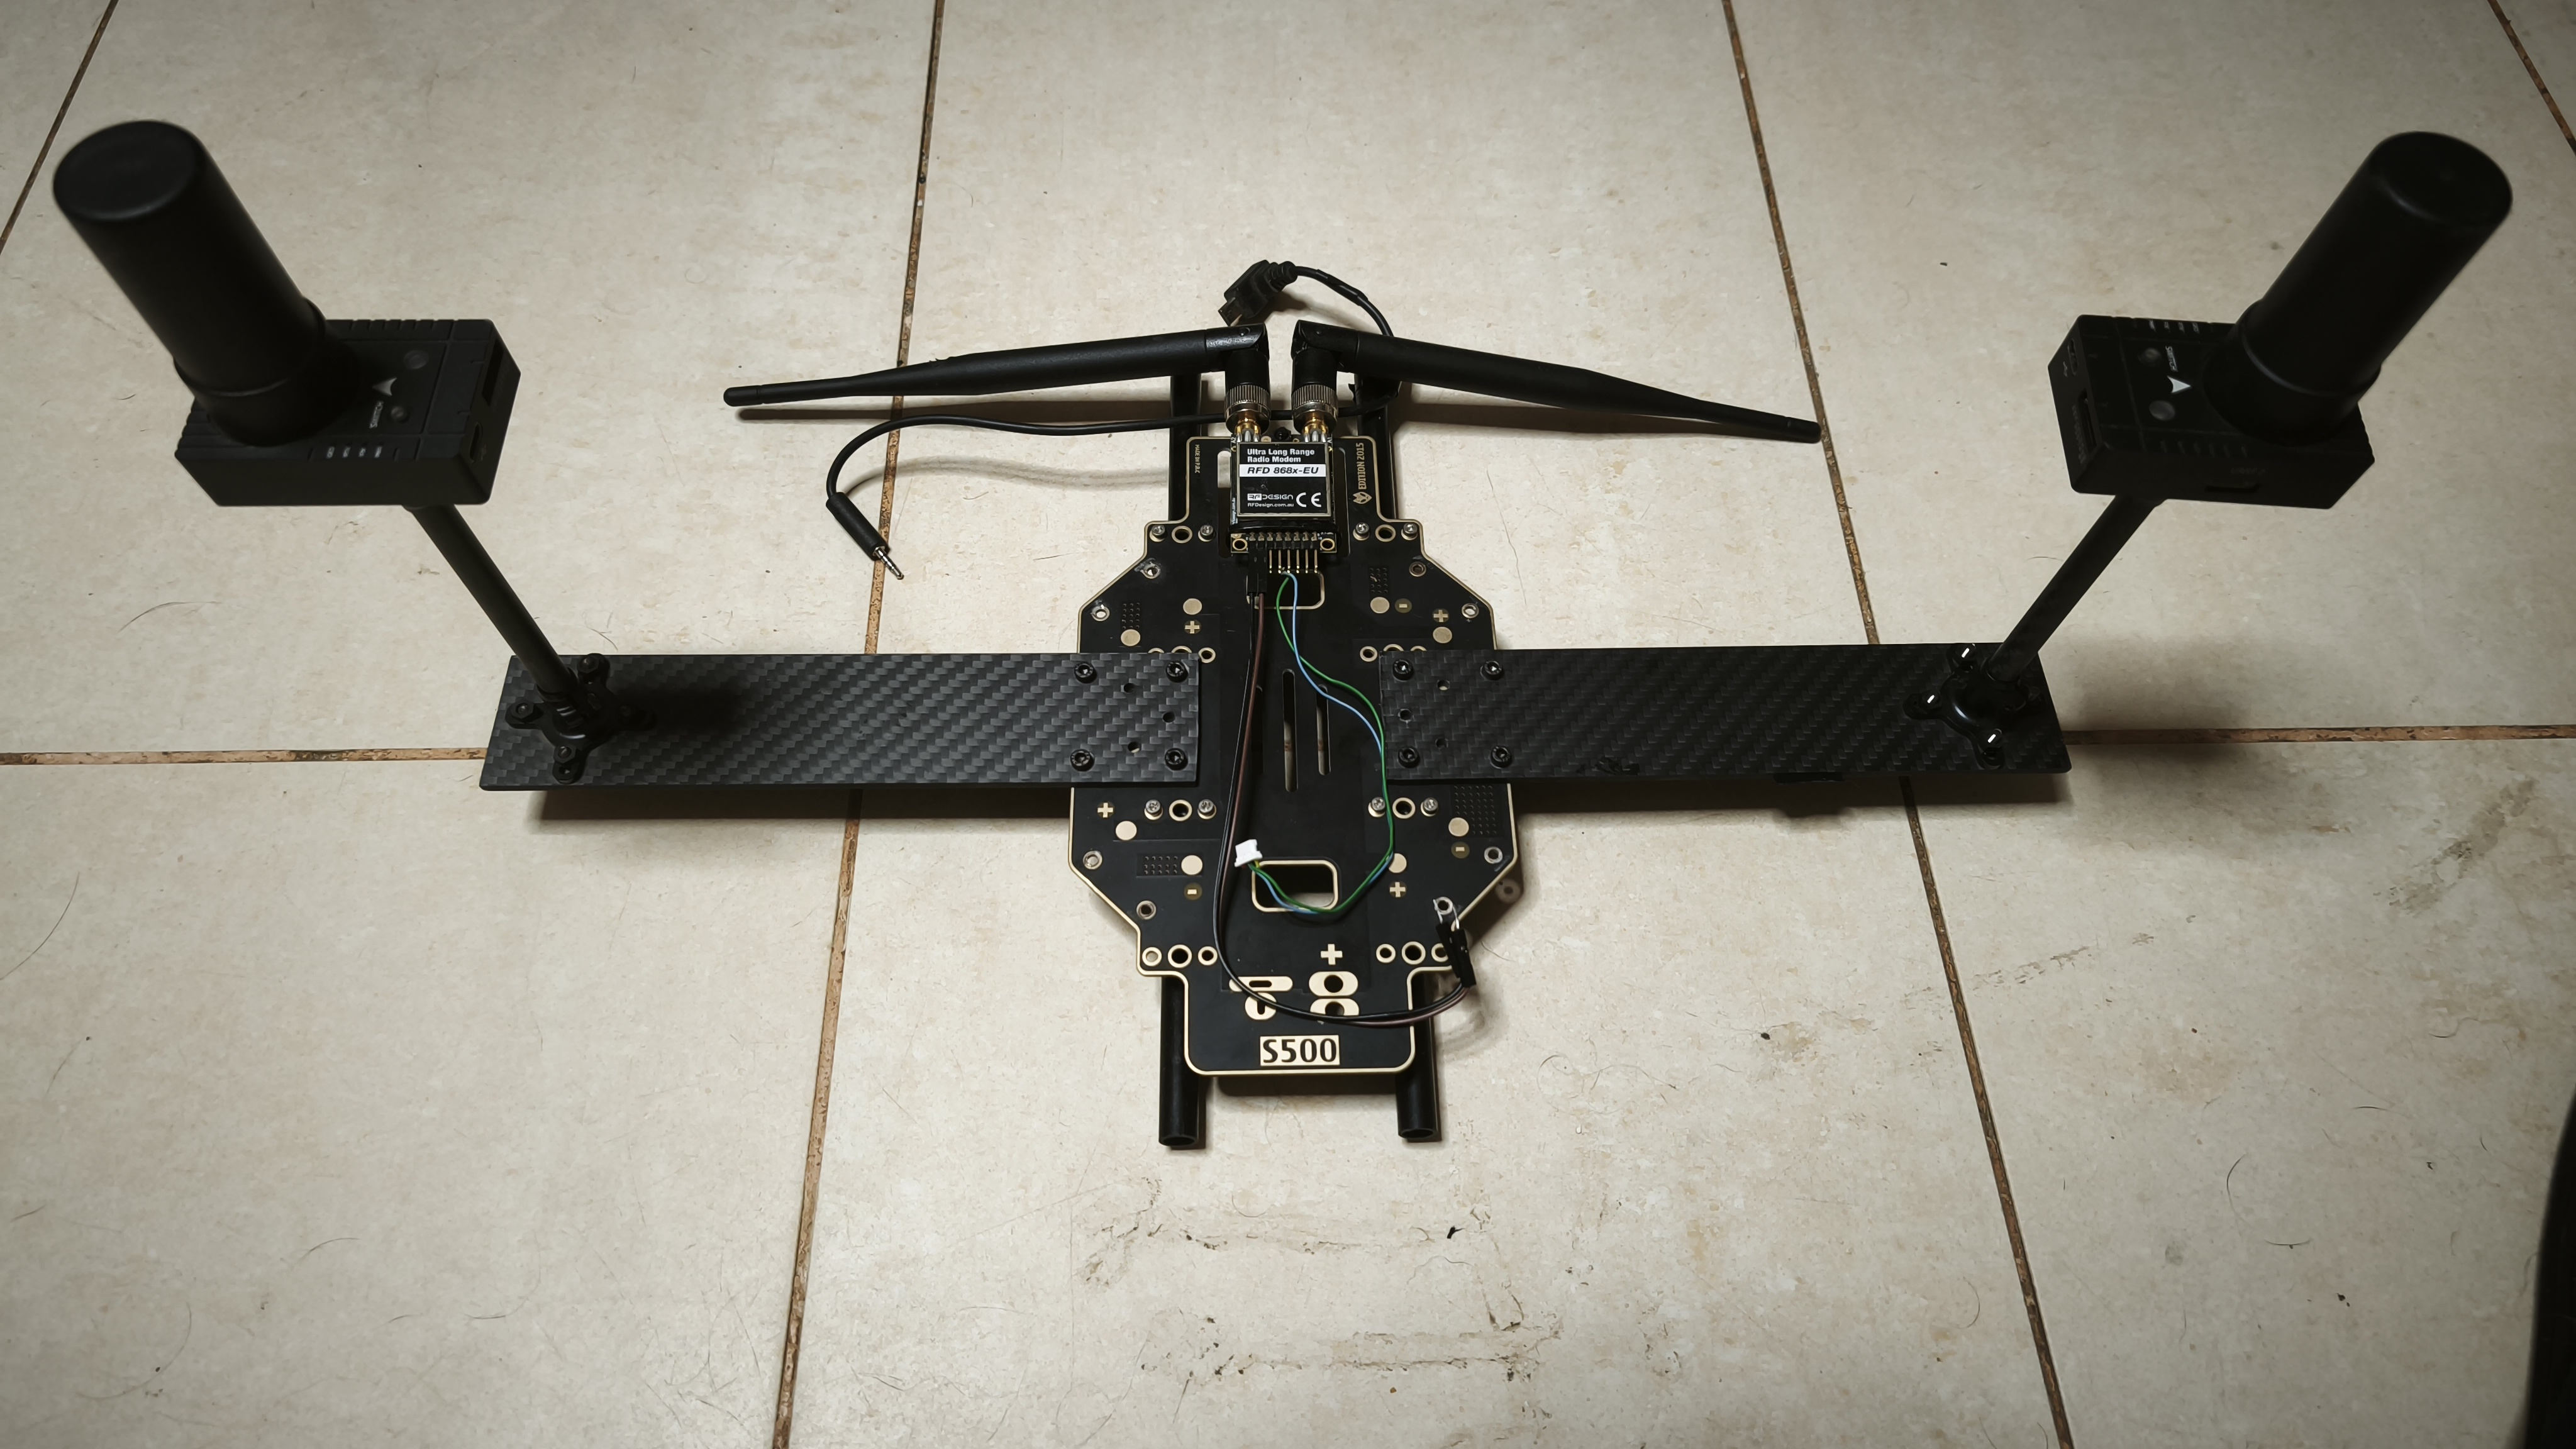
\includegraphics[width=\textwidth]{img/xasis_base.jpg}
    \caption{S500 central board with the carbon \emph{bracket}, the two H-RTK F9P Helical modules on vertical posts and the RFD868x module.}
    \label{fig:xassis-base}
\end{figure}

\begin{figure}[H]
    \centering
    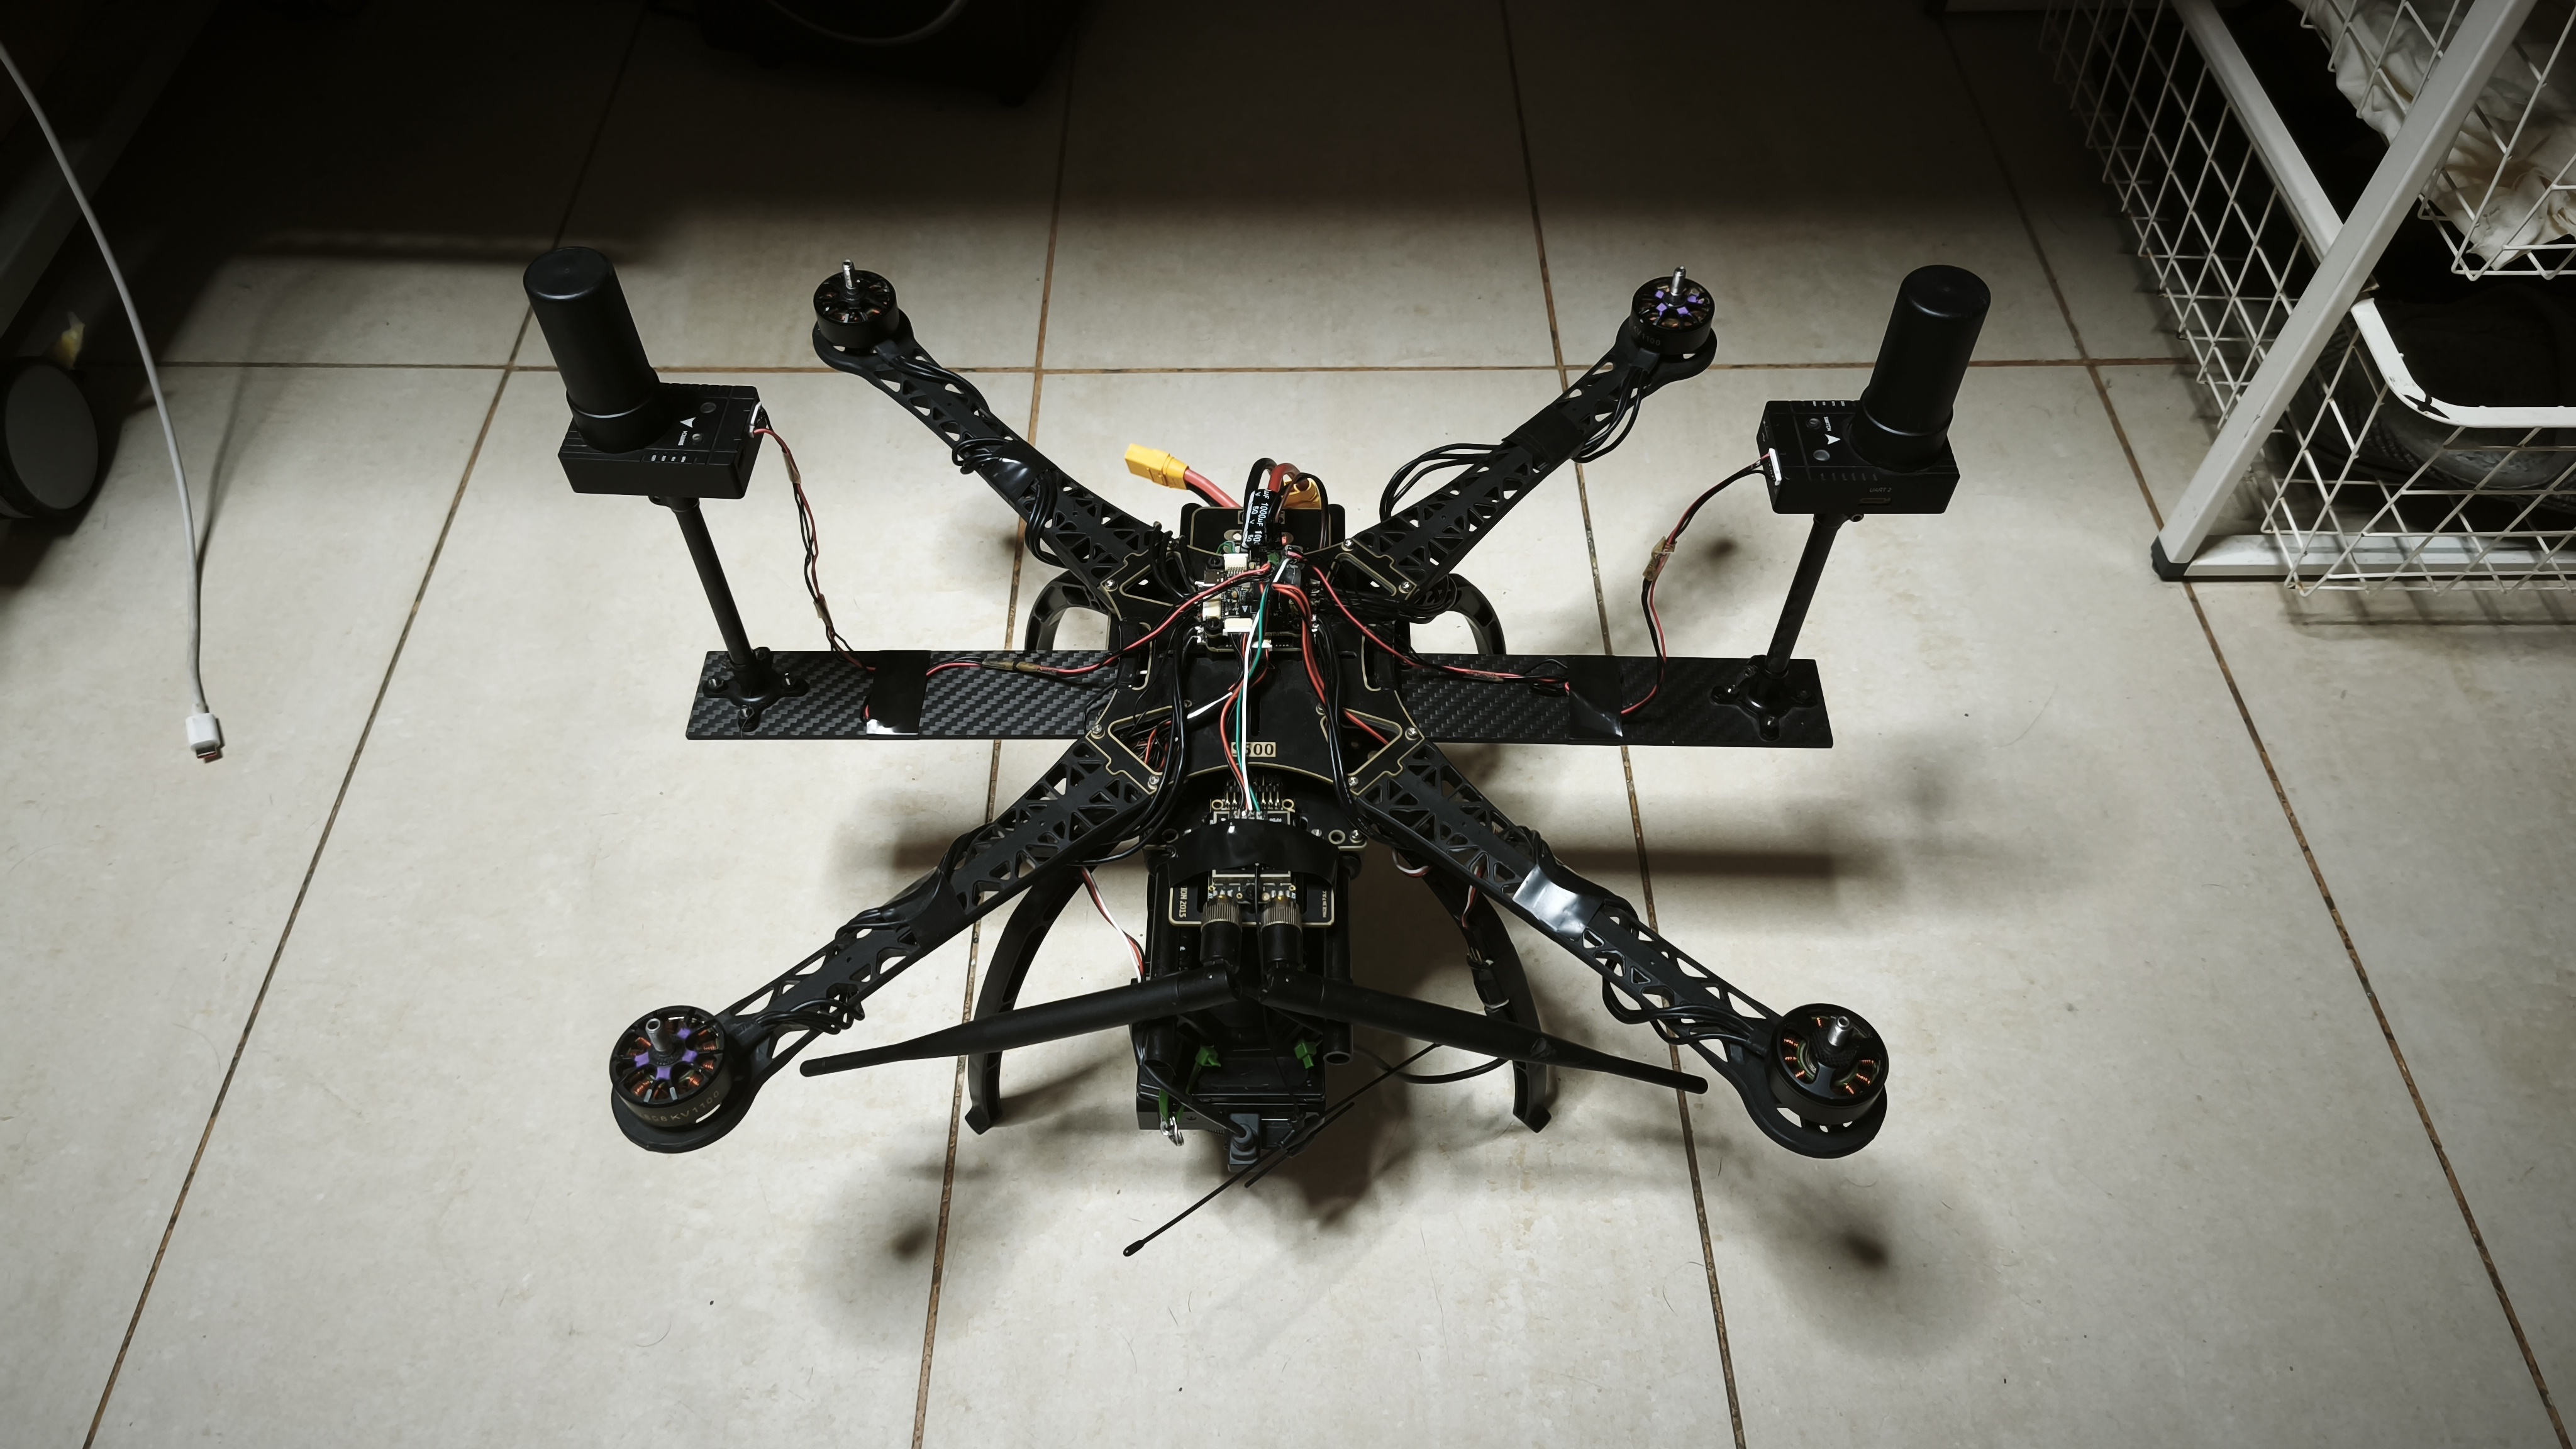
\includegraphics[width=\textwidth]{img/xasis_sencer.jpg}
    \caption{Finished drone seen from above: motors, lateral \emph{baseline} with the two GNSS antennas, telemetry module and landing gear.}
    \label{fig:xassis-sencer}
\end{figure}

Under the \emph{frame} there is a rail made of two parallel carbon bars with clamps (\cref{fig:xassis-abaix}), which supports both the camera and the battery. The camera (Sony $\alpha$6000 with the 25~mm lens) points at nadir, with the Seagull SYNC2 on the hot shoe; the 6S battery is fixed to the same rail, so that the centre of gravity is close to the vertical axis of the drone.

\begin{figure}[H]
    \centering
    \begin{subfigure}[b]{0.49\textwidth}
        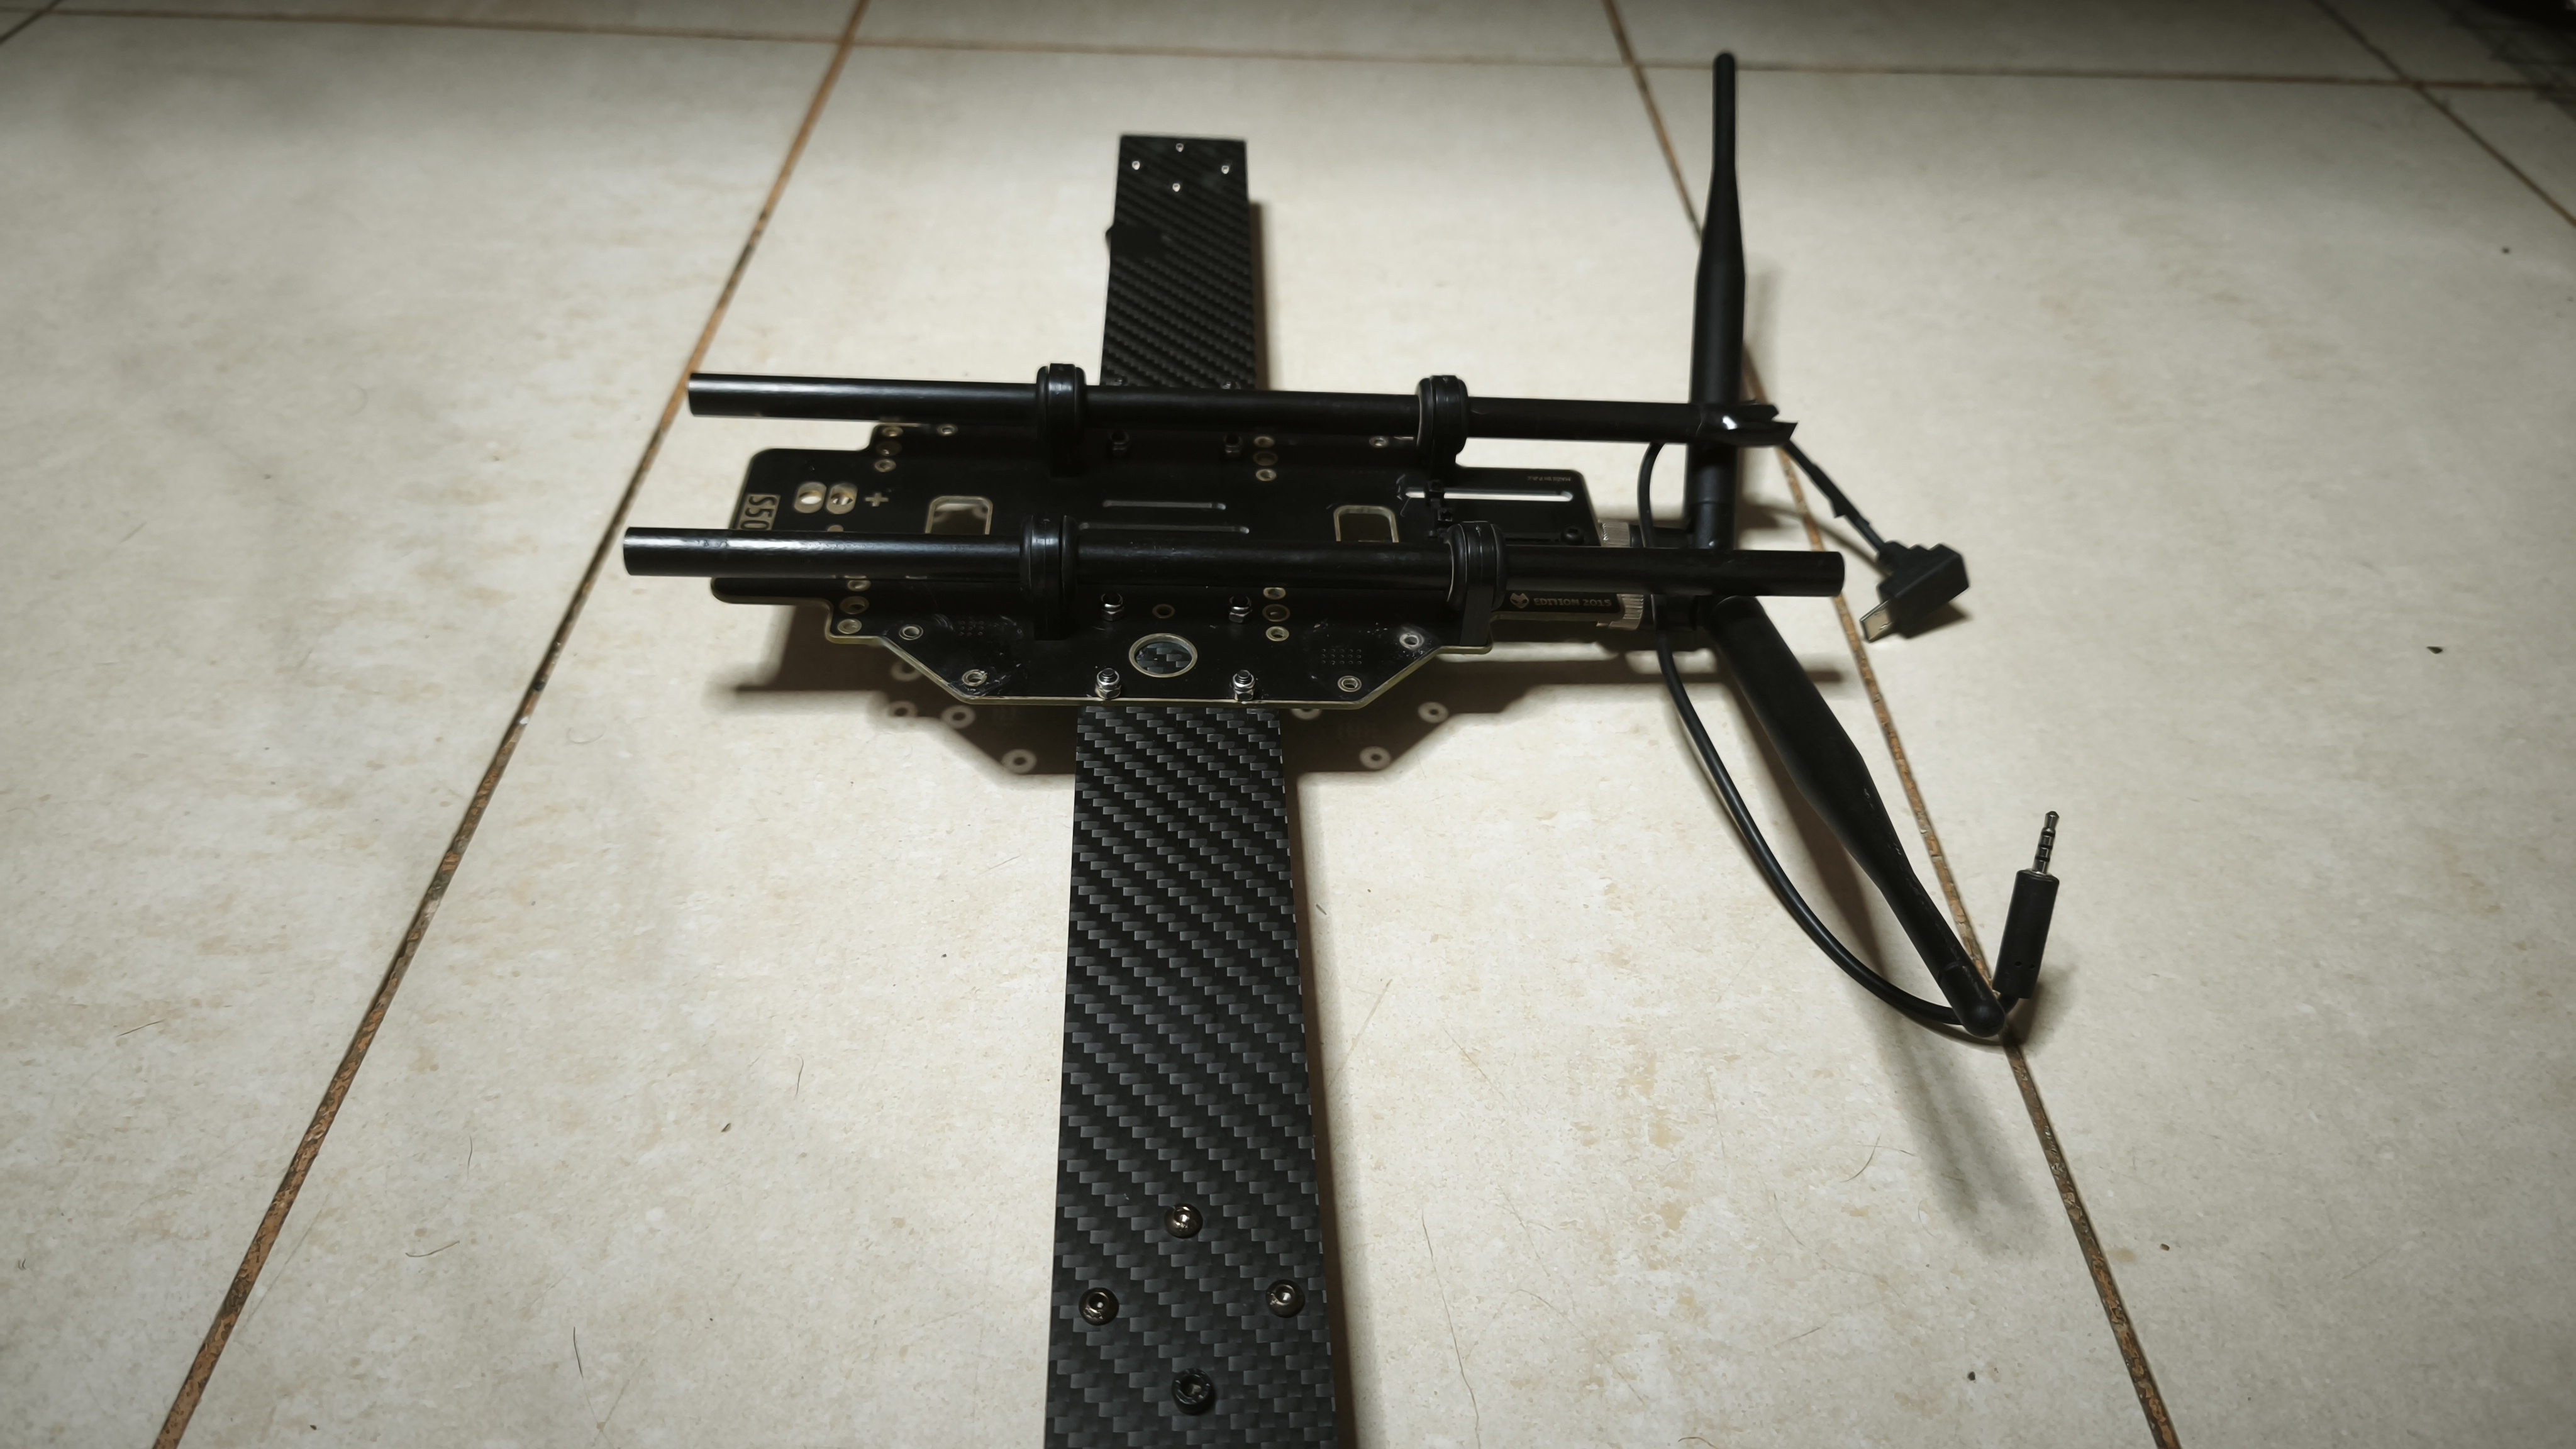
\includegraphics[width=\textwidth]{img/xasis_abaix_buit.jpg}
        \caption{Lower rail without load.}
    \end{subfigure}
    \hfill
    \begin{subfigure}[b]{0.49\textwidth}
        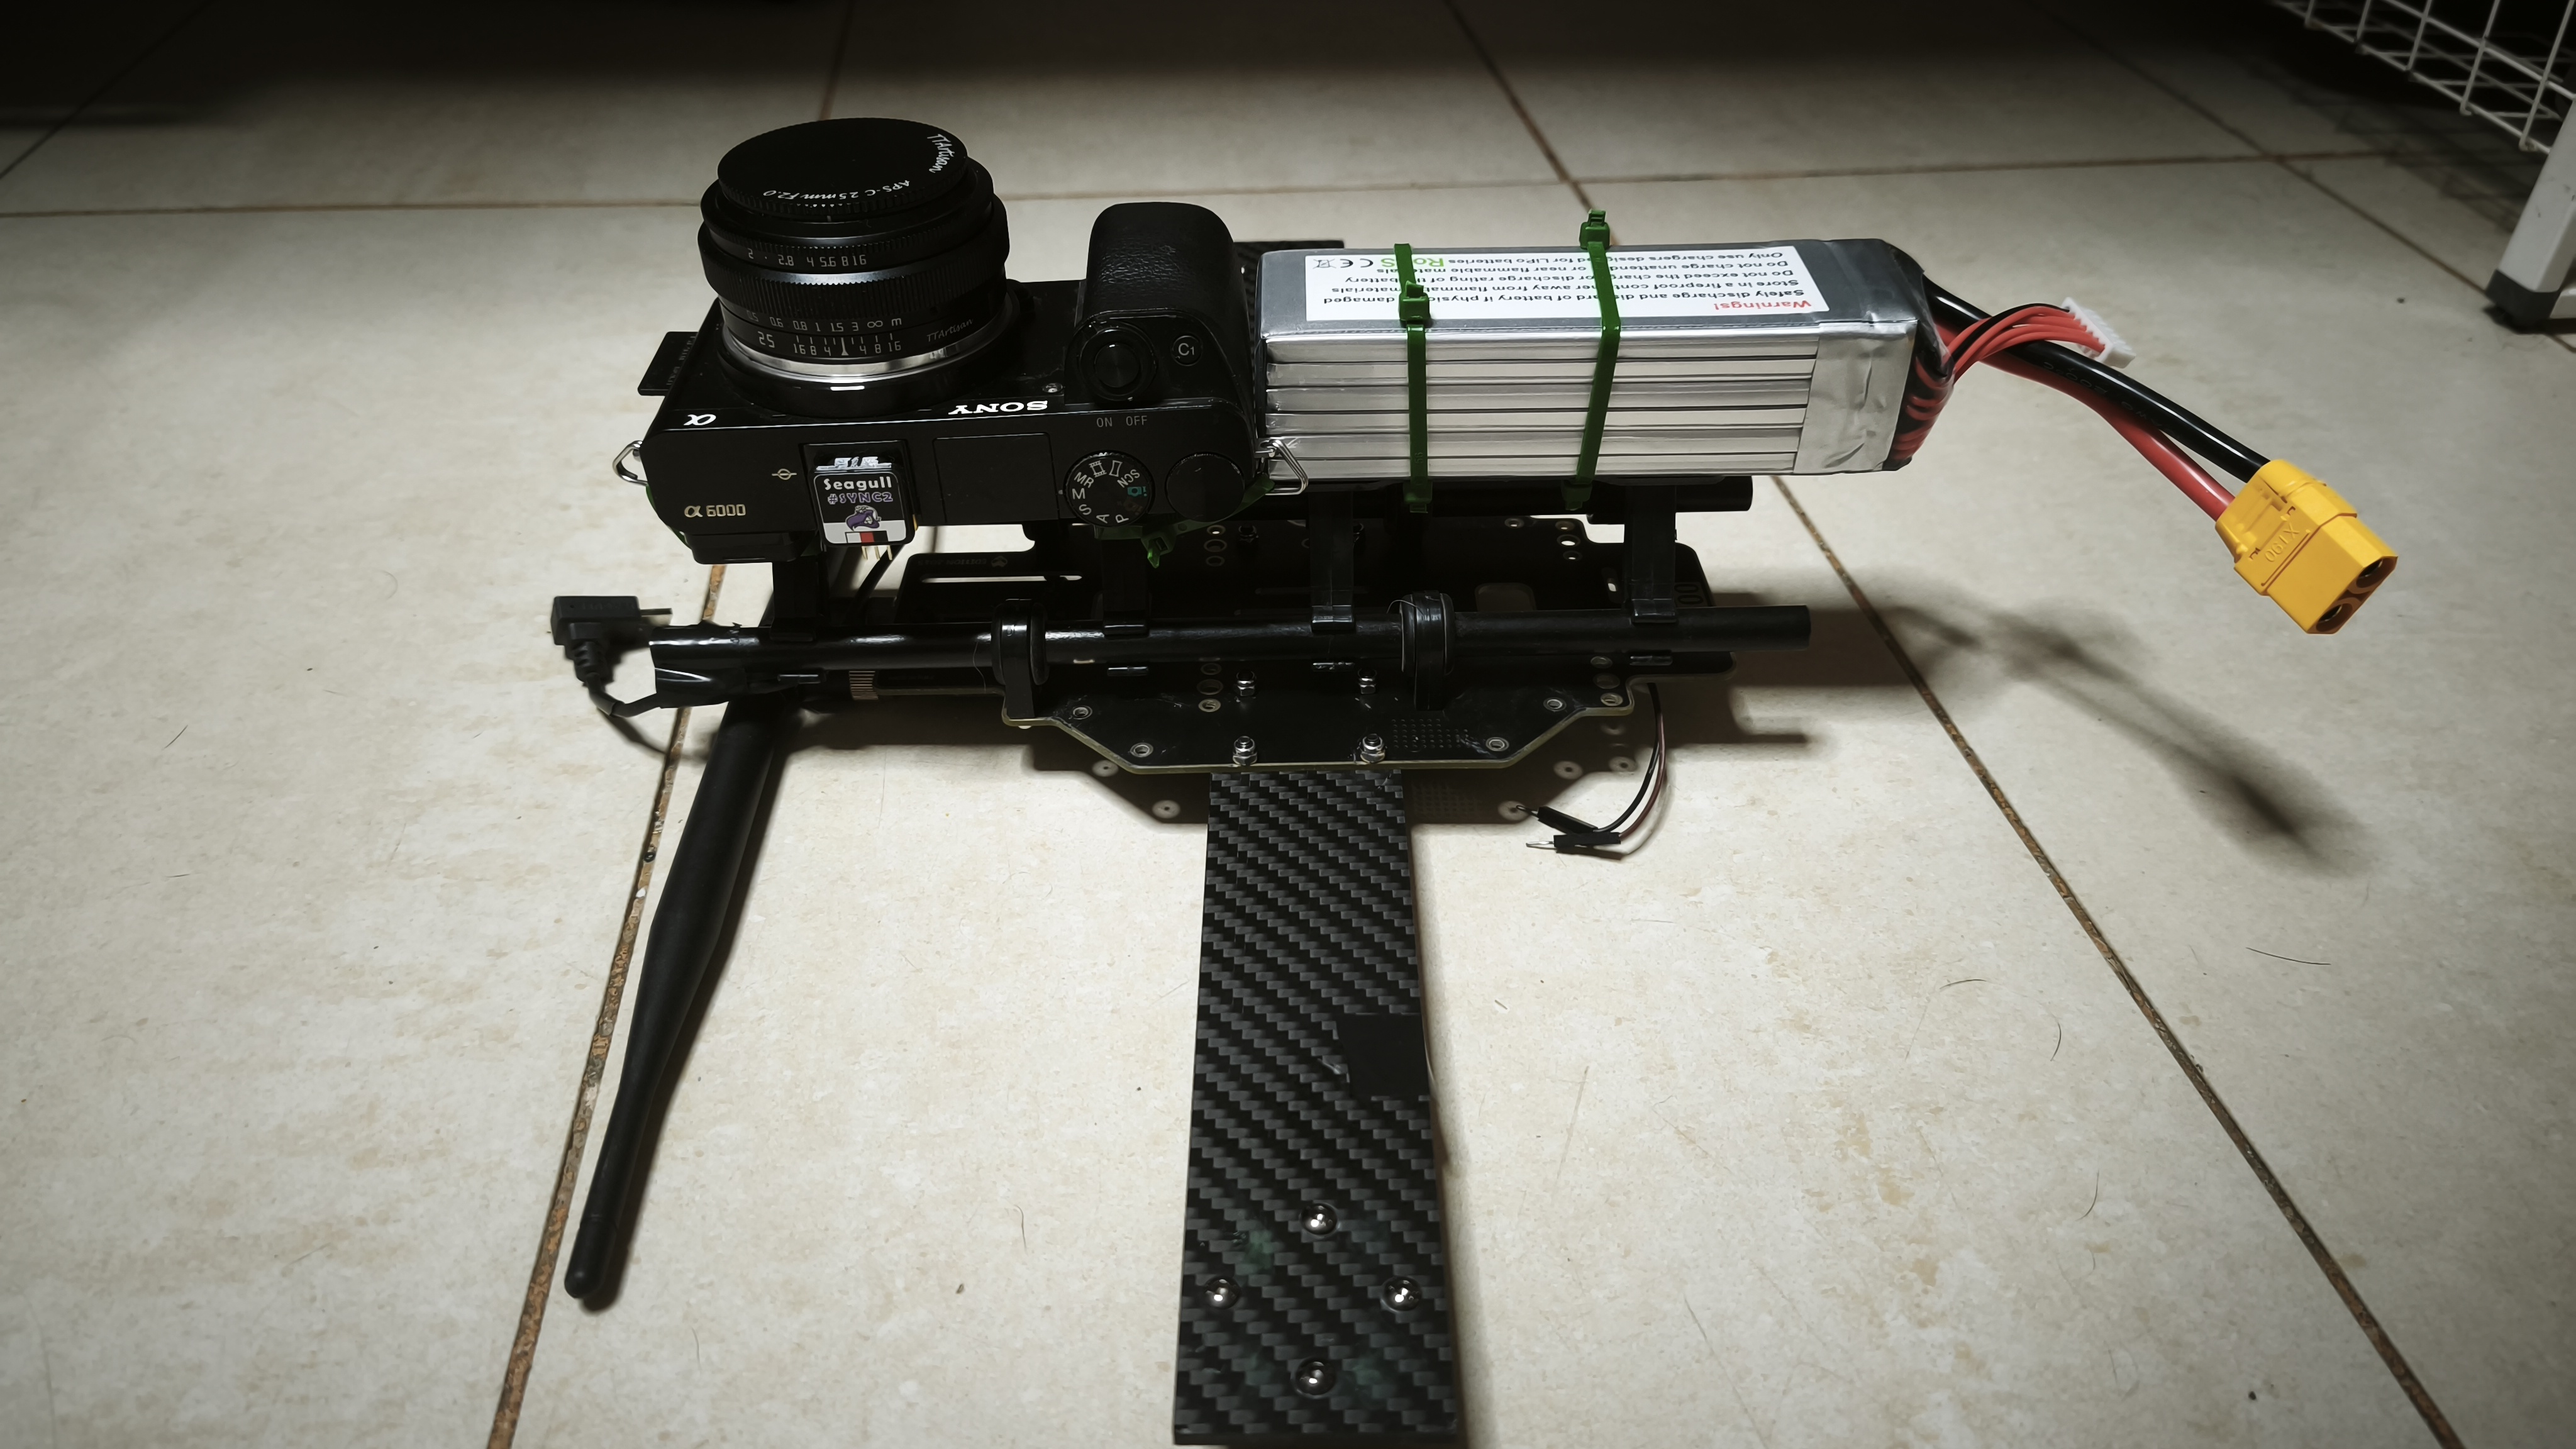
\includegraphics[width=\textwidth]{img/xasis_abaix_ple.jpg}
        \caption{With the camera, the SYNC2 and the battery.}
    \end{subfigure}
    \caption{Bottom view of the \emph{frame} (turned over): carbon rail and camera module.}
    \label{fig:xassis-abaix}
\end{figure}

The configuration of the FC serial ports and the \emph{firmware} parameters (camera, \emph{moving baseline} GPS) are described in the operation manual (\cref{chap:manual}).

\subsubsection*{Electrical connections}

\Cref{fig:connexions} shows the wiring of the drone and \cref{tab:connexions} summarises it pad by pad. All devices connect directly to pads of the flight controller; no GNSS receiver shares a cable with the other (the \emph{moving baseline} stream goes through the controller, \cref{subsec:gps-moving-baseline}).

\begin{figure}[p]
    \centering
    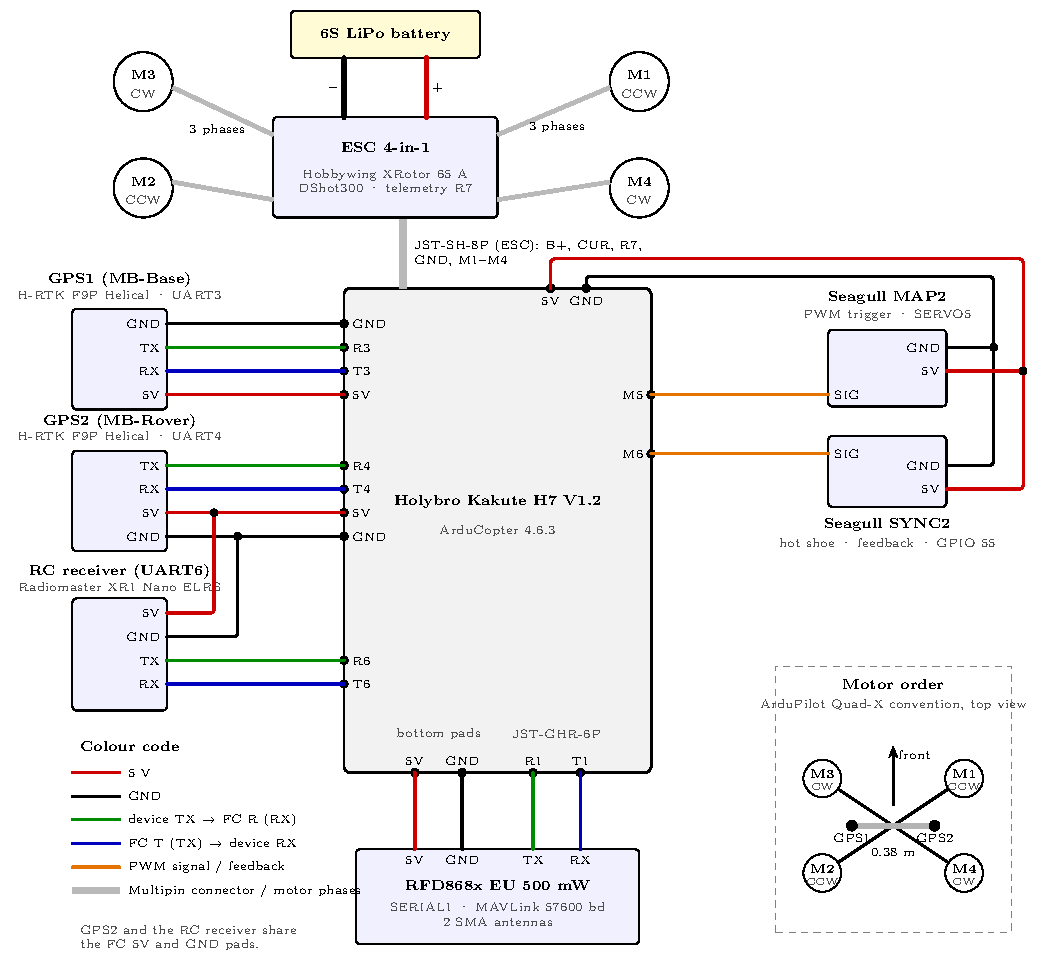
\includegraphics[width=\textwidth]{img/diagrama_connexions_en.pdf}
    \caption{Connection diagram of the drone. The colours follow the legend: green for the TX line of the device towards the RX of the FC and blue for the TX of the FC towards the RX of the device.}
    \label{fig:connexions}
\end{figure}

\begin{table}[H]
    \centering
    \caption{Flight controller connections (Kakute H7 V1.2)}
    \label{tab:connexions}
    \small
    \begin{tabular}{P{3.2cm}P{3.9cm}P{3.5cm}P{2.6cm}}
        \toprule
        Device & FC pads & Function & ArduPilot port \\
        \midrule
        GPS1 (MB-Base) & R3, T3, 5V, GND & UART & \texttt{SERIAL3} \\
        GPS2 (MB-Rover) & R4, T4, 5V, GND & UART & \texttt{SERIAL4} \\
        ELRS receiver & R6, T6, 5V, GND & UART (CRSF) & \texttt{SERIAL6} \\
        RFD868x & R1, T1 (JST-GHR-6P); 5V, GND & UART (MAVLink) & \texttt{SERIAL1} \\
        4-in-1 ESC & JST-SH-8P: B+, CUR, R7, GND, M1--M4 & DShot, voltage, current, telemetry & \texttt{SERIAL7} \\
        Seagull MAP2 & M5; 5V, GND & \emph{trigger} PWM & \texttt{SERVO5} \\
        Seagull SYNC2 & M6; 5V, GND & hot-shoe \emph{feedback} & \texttt{SERVO6} (GPIO 55) \\
        \bottomrule
    \end{tabular}
\end{table}

\subsection{GNSS base}
\label{subsec:muntatge-base}

The base is a compact stack of three boards fixed to one leg of the tripod with clamps (\cref{fig:base}): the ArduSimple simpleRTK2B Pro receiver (with the ZED-F9P), the Raspberry Pi Zero W and the Waveshare UPS HAT with the two 18650 batteries. The BD900 GNSS antenna is mounted levelled, with a ground plane, on the 5/8-inch thread of the survey tripod, at a height of 122~cm in the flight tests.

The connections are (\cref{fig:base-connexions}):
\begin{itemize}
    \item \textbf{Antenna $\rightarrow$ simpleRTK2B Pro:} coaxial cable with SMA connector.
    \item \textbf{simpleRTK2B Pro $\rightarrow$ Raspberry Pi:} one USB-C cable, which carries the data (RTCM3 corrections and receiver configuration) and powers the receiver from the Pi.
    \item \textbf{UPS HAT $\rightarrow$ Raspberry Pi:} only the power pins of the Pi header are connected to the UPS HAT, which powers it from the batteries; there is no communication line between the two.
\end{itemize}

\begin{figure}[H]
    \centering
    \begin{tikzpicture}[box/.style={draw, rounded corners=2pt, align=center, font=\small, minimum height=10mm, minimum width=22mm, fill=blue!5},
        arr/.style={-{Stealth[length=2mm]}, thick}, node distance=17mm]
        \node[box] (ant) {Multiband\\antenna};
        \node[box, right=of ant] (rtk) {simpleRTK2B Pro\\(ZED-F9P)};
        \node[box, right=of rtk] (pi) {Raspberry Pi\\Zero W};
        \node[box, right=of pi] (ups) {UPS HAT\\2$\times$18650};
        \draw[arr] (ant) -- node[above, font=\scriptsize] {coaxial SMA} (rtk);
        \draw[arr] (rtk) -- node[above, font=\scriptsize] {USB-C} (pi);
        \draw[arr] (ups) -- node[above, font=\scriptsize] {5~V pins} (pi);
    \end{tikzpicture}
    \caption{RTK base connections: antenna, receiver, SBC and power.}
    \label{fig:base-connexions}
\end{figure}

\begin{figure}[H]
    \centering
    \begin{subfigure}[b]{0.43\textwidth}
        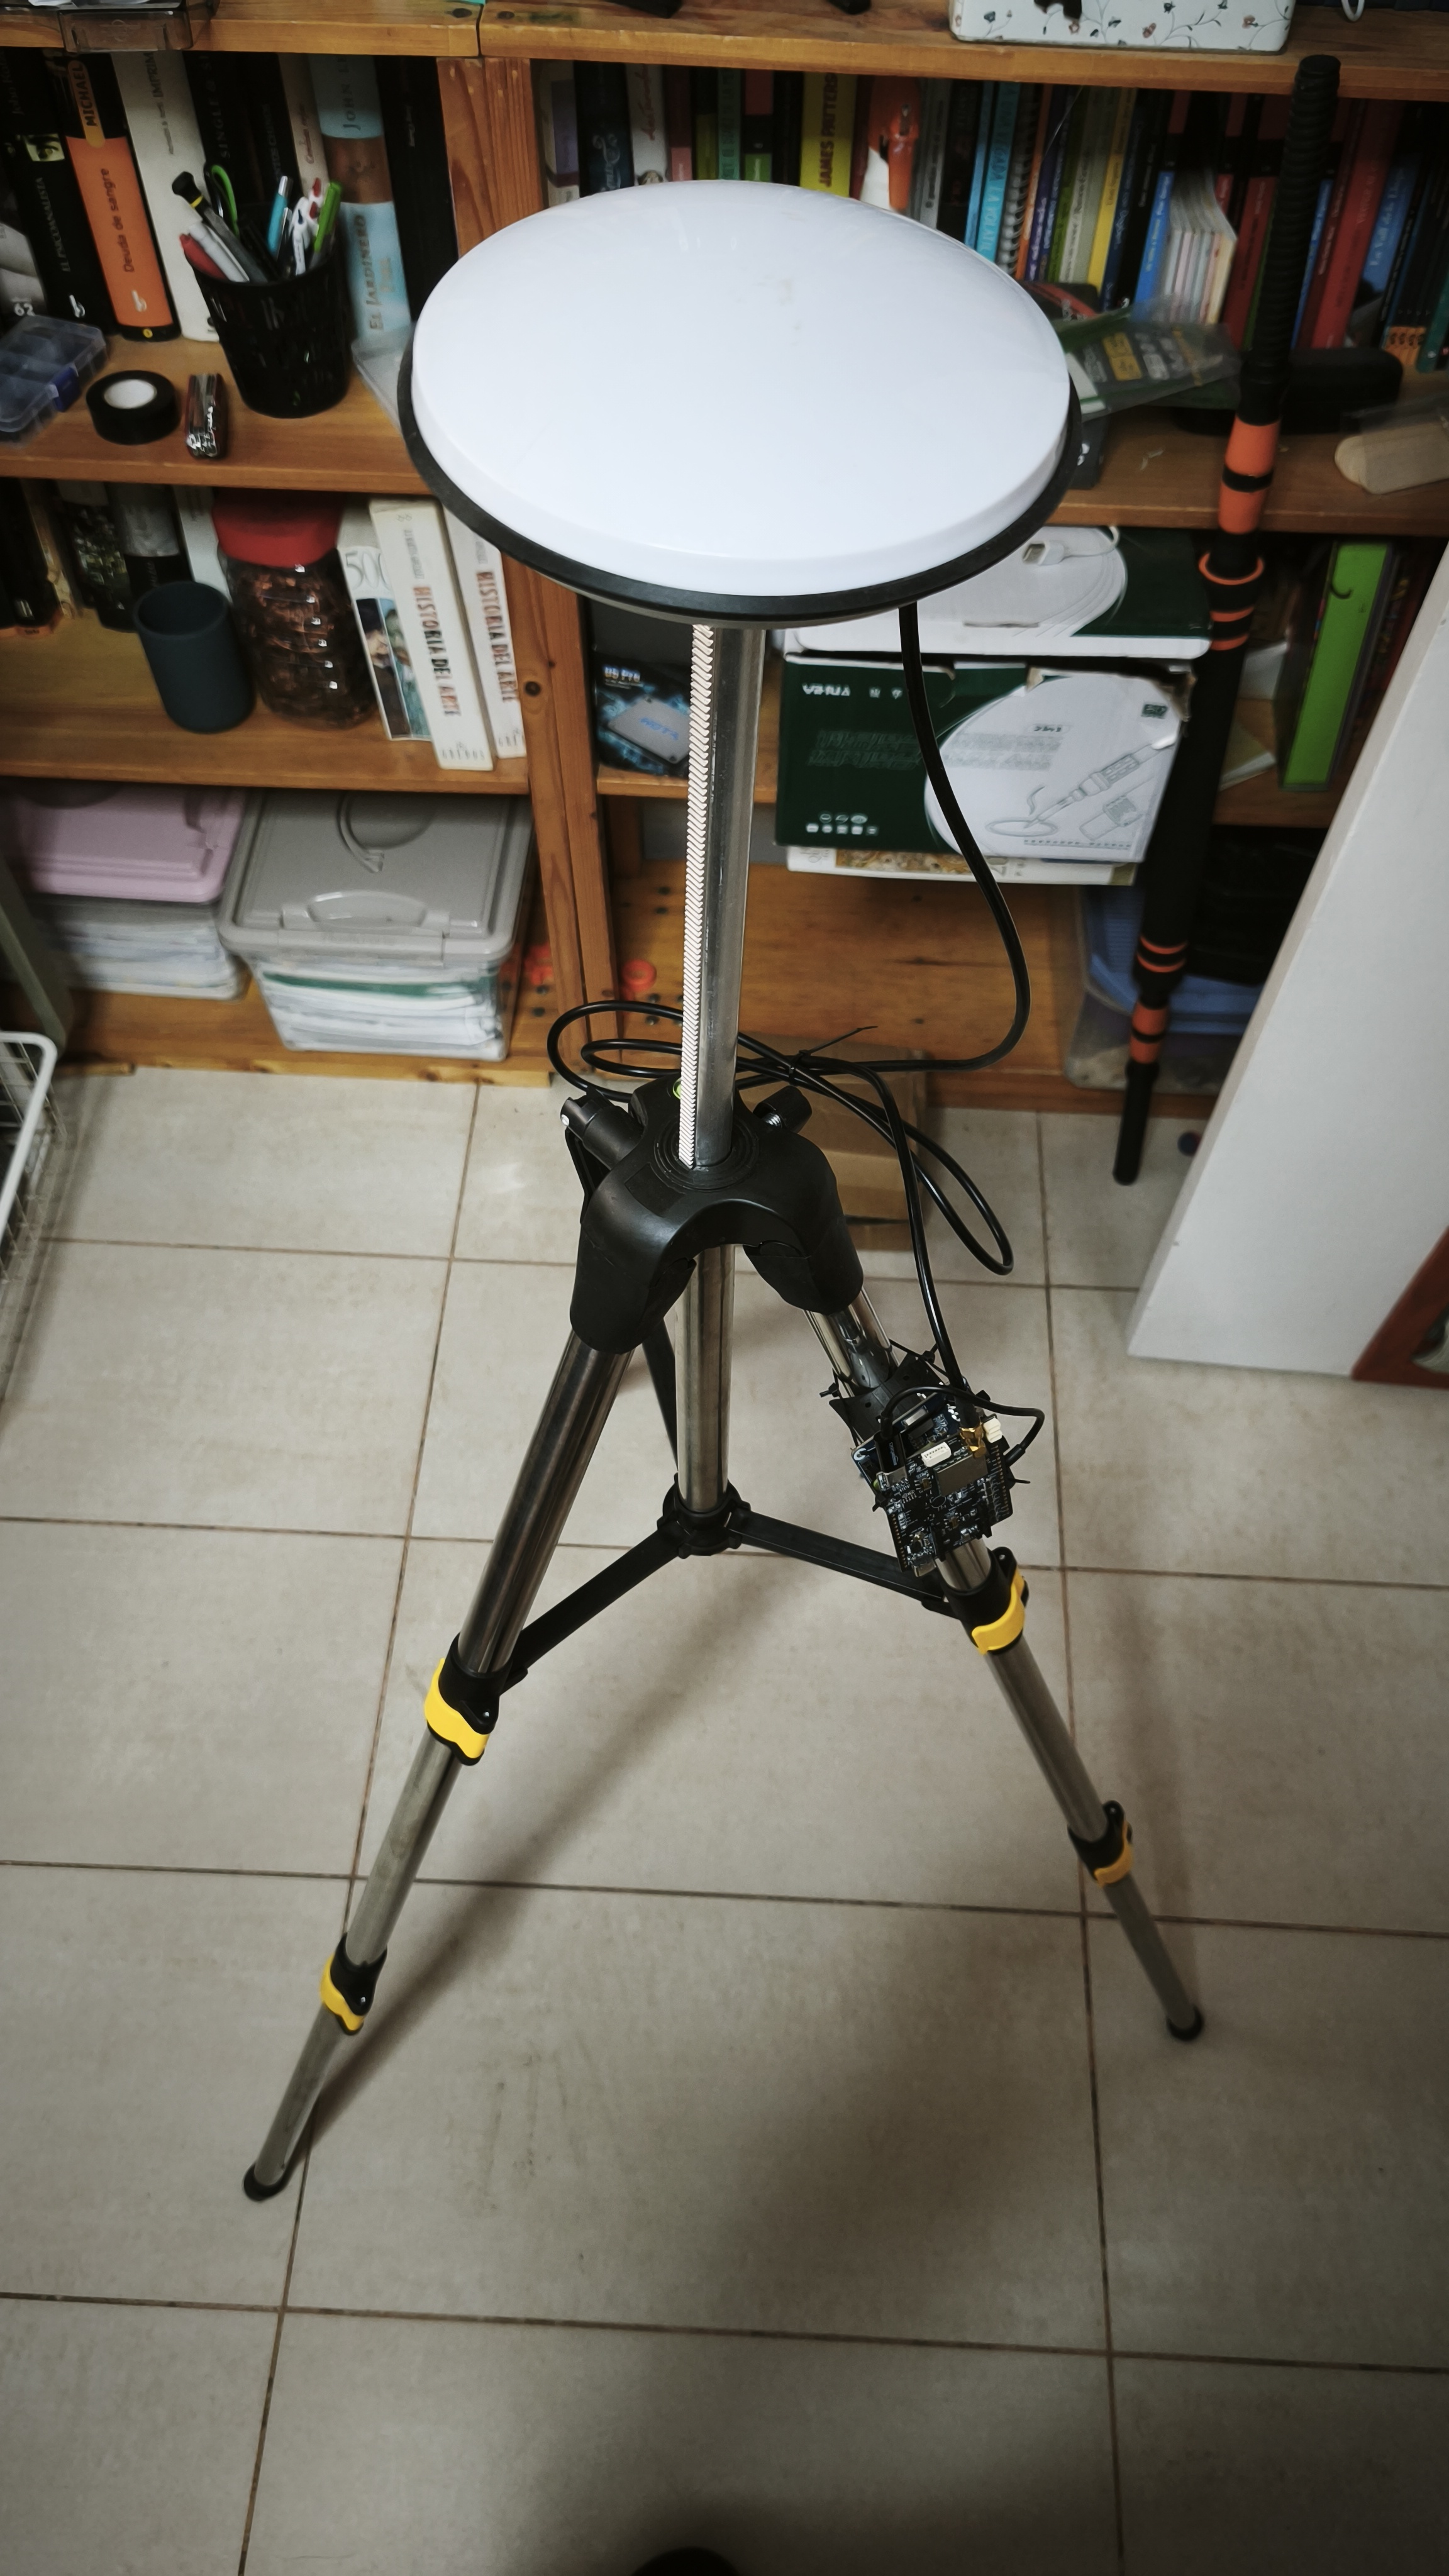
\includegraphics[width=\textwidth]{img/Base_sencera.jpg}
        \caption{Complete base on the tripod.}
    \end{subfigure}
    \hfill
    \begin{subfigure}[b]{0.43\textwidth}
        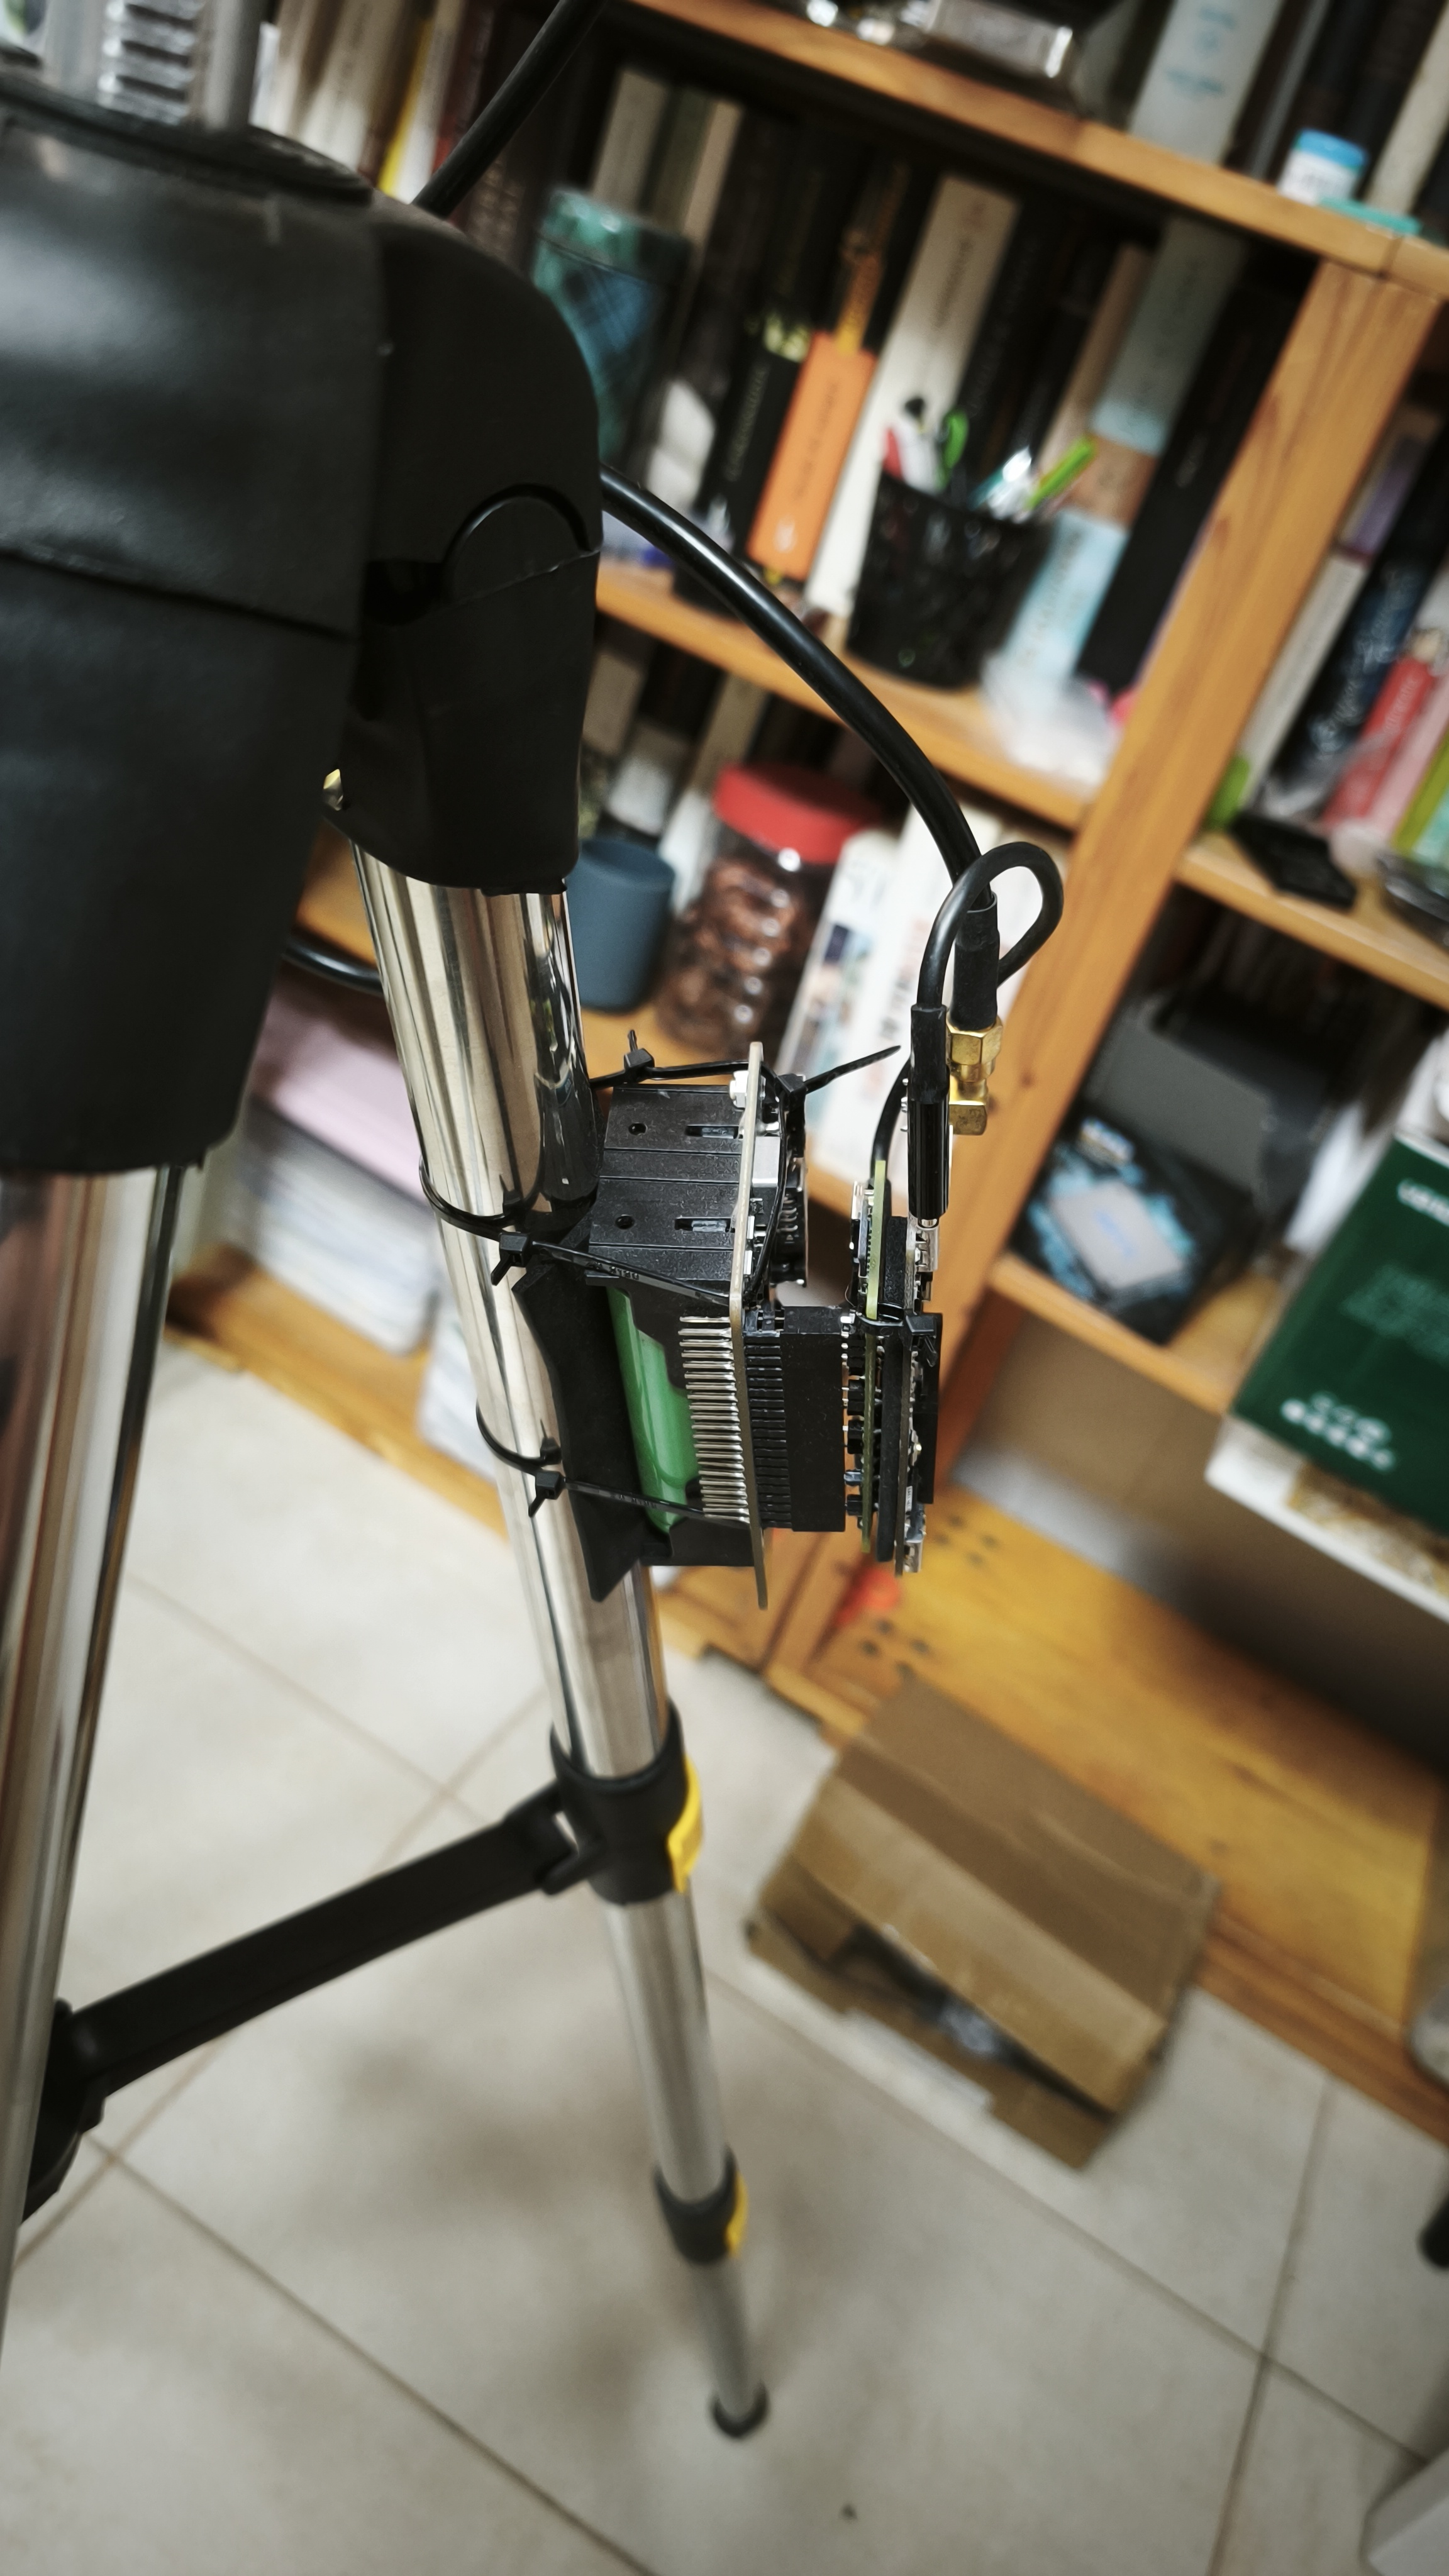
\includegraphics[width=\textwidth]{img/Stack_base.jpg}
        \caption{Base stack fixed to a leg.}
    \end{subfigure}
    \caption{RTK base: multiband antenna on the tripod and stack with the simpleRTK2B Pro, the Raspberry Pi and the UPS HAT.}
    \label{fig:base}
\end{figure}

The procedure for positioning the base and fixing its coordinates is described in \cref{sec:protocol-camp}.

\paragraph{Software and configuration.} The Raspberry Pi runs Raspberry Pi OS (Debian~13, 32-bit). The corrections are distributed by the RTKLIB \texttt{str2str} program (the \texttt{rtklibexplorer} fork, compiled on the Pi itself), run as a \texttt{systemd} service that starts with the board. The service is called \texttt{rtkbase}, but it has no relation to the \texttt{rtkbase} project in the bibliography: it reads the USB serial port of the receiver (115,200~bd) and opens a TCP server on port 5000 that forwards the receiver stream as it comes out (RTCM3 and the UBX navigation messages that it emits on the same port), without NTRIP. Besides forwarding it, the service saves it to a file for the whole session (\cref{sec:protocol-camp}). The GS connects to it with Mission Planner's \emph{RTK/GPS Inject} in \emph{TCP Client} mode, at \texttt{192.168.4.1:5000}.

The WiFi access point (\texttt{BaseRTK}) is managed by NetworkManager in \emph{shared} mode: 2.4~GHz band, channel~6, WPA-PSK, address \texttt{192.168.4.1/24} with DHCP, and it is activated at every boot. PMF (802.11w) must be disabled, because the \texttt{brcmfmac} driver of the Pi does not support it in AP mode.

The ZED-F9P (\emph{firmware} HPG~1.51, protocol~27.50) is configured with \texttt{ubxtool}: NMEA disabled on the USB port, RTCM3 enabled and messages 1005, 1074, 1084, 1094, 1124 and 1230 at 1~Hz. The total stream on port 5000, with the UBX navigation messages that the receiver also emits, was about 15~kbps. The base position is not fixed: the receiver runs a \emph{survey-in} in every session, with 300~s as a minimum and until the precision of the mean is 2~m or better, and the configuration is kept in the \emph{flash} memory of the receiver. Flight tests 5 and 6 used this base and this method, with the antenna at 122~cm.

\textbf{Limitation.} In flight tests 5 and 6 the service only forwarded the stream, without saving it, and the position resulting from the \emph{survey-in} was not noted down; therefore the absolute position of those flights cannot be recovered. Since every session performs a new one, the absolute position of the map has a common error of the order of metres; this shifts the whole map but does not change its relative geometry. Since 27 October 2026 the service saves the stream of every session, so the position can be computed afterwards (\cref{sec:protocol-camp}).

\section{System status}
\label{sec:estat-actual}

The hardware is complete and the system has accumulated about 30~minutes of flight according to the controller counter, spread between the tuning campaign (\cref{chap:proves-vol}) and two photogrammetry flights (\cref{chap:vols-prova}). With the current configuration the drone flies with RTK Fixed on both receivers and valid GNSS \emph{yaw}, and the photographic chain (distance-based triggering, hot-shoe \emph{feedback}, geotagging and processing) is operational end to end. The current limitations --~above all the endurance and the absolute validation with control points~-- are collected in \cref{sec:balanc-vols,sec:autonomia}, and the pending work is in \cref{sec:pendents-proves-vol}.
